\documentclass[svgnames]{beamer}

\usepackage{pri}

\graphicspath{{./}{figures/}{figures/12-indexing-figs/}} 

\subtitle{Efficient Index Construction}


\begin{document}

\maketitle
\makeoutline

\begin{frame}
    \frametitle{Bibliography}
    
    Managing Gigabytes: Compressing and Indexing Documents and Images - 2nd
    edition Ian H. Witten, Alistair Moffat, Timothy C. Bell Morgan Kaufmann
    2000

\end{frame}

\section{Basic Concepts}

\begin{frame}
    \frametitle{Text Indexes}

    \begin{block}{}
        \begin{itemize}
        \item An index is a mechanism to locate a given term in the \emph{document
              collection}
        \item Index types:
            \begin{itemize}
            \item \alert{inverted files}
            \item signature files
            \item bitmaps
            \end{itemize}
        \end{itemize}
    \end{block}

\end{frame}

% ----------------------------------------------------------------------

\begin{frame}
    \frametitle{Definitions}

    \begin{block}{}
        \begin{itemize}
        \item A \emph{document collection} is a set of separate documents
        \item Documents are composed of \emph{terms}
        \item Indexes provide efficient access to the documents given one or more
            terms
        \item Indexes can have different \emph{granularities}:
            \begin{itemize}
            \item set of documents $\rightarrow$ document $\rightarrow$ $\cdots$
                $\rightarrow$ paragraph $\rightarrow$ word
            \end{itemize}
        \end{itemize}
    \end{block}

\end{frame}

% ----------------------------------------------------------------------

\newcounter{num}
\setcounter{num}{0}
\newcommand{\inum}{\addtocounter{num}{1}\thenum}

\begin{frame}
    \frametitle{A Document Collection}
    
    \begin{block}{}
        \small
        \begin{tabular}{rl}
            Doc. & Text \\\hline
            \inum & That government is best which governs least \\
            \inum & That government is best which governs not at all \\
            \inum & The mass of men serve the state not as men, \\
            & but as machines \\
            \inum & Wooden men can be manufactured that will serve the \\
            & purpose as well \\
            \inum & Government is at best but an expedient \\
            \inum & But most governments are usually inexpedient \\
        \end{tabular}
    \end{block}

\end{frame}

% ----------------------------------------------------------------------

\begin{frame}
    \frametitle{An Inverted File}
    
    \small

    \begin{columns}
        \column{0.49\textwidth}

        \setcounter{num}{0}
        \begin{block}{Lexicon}
            \centering
            \begin{tabular}{rl}
                Num. & Term \\\hline
                \inum & best \\
                \inum & expedient \\
                \inum & government \\
                \inum & governs \\
                \inum & inexpedient \\
                \inum & least \\
                \inum & machines \\
                \inum & manufactured \\
                \inum & mass \\
                \inum & men \\
                \inum & purpose \\
                \inum & serve \\
                \inum & state \\
                \inum & wooden \\
            \end{tabular}
        \end{block}

        \column{0.49\textwidth}

        \setcounter{num}{0}
        \begin{block}{Inverted file}
            \centering
            \begin{tabular}{rl}
                Num. & Inverted list \\\hline
                \inum & $\langle 3;1,2,5\rangle$ \\
                \inum & $\langle 1;5\rangle$ \\
                \inum & $\langle 4;1,2,5,6\rangle$ \\
                \inum & $\langle 2;1,2\rangle$ \\
                \inum & $\langle 1;6\rangle$ \\
                \inum & $\langle 1;1\rangle$ \\
                \inum & $\langle 1;3\rangle$ \\
                \inum & $\langle 1;4\rangle$ \\
                \inum & $\langle 1;3\rangle$ \\
                \inum & $\langle 2;3,4\rangle$ \\
                \inum & $\langle 1;4\rangle$ \\
                \inum & $\langle 2;3,4\rangle$ \\
                \inum & $\langle 1;3\rangle$ \\
                \inum & $\langle 1;4\rangle$ \\        
            \end{tabular}
        \end{block}

    \end{columns}

\end{frame}

% ----------------------------------------------------------------------

\begin{frame}
    \frametitle{Inverted file with word granularity}

    \small
    
    \setcounter{num}{0}
    \begin{block}{Inverted File}
        \centering
        \begin{tabular}{rl}
            Num. & Inverted list \\\hline
            \inum & $\langle 3;(1;4),(2;4),(5;4)\rangle$ \\
            \inum & $\langle 1;(5;7)\rangle$ \\
            \inum & $\langle 4;(1;2),(2;2),(5;1),(6;3)\rangle$ \\
            \inum & $\langle 2;(1;6),(2;6)\rangle$ \\
            \inum & $\langle 1;(6;6)\rangle$ \\
            \inum & $\langle 1;(1;7)\rangle$ \\
            \inum & $\langle 1;(3;13)\rangle$ \\
            \inum & $\langle 1;(4;5)\rangle$ \\
            \inum & $\langle 1;(3;2)\rangle$ \\
            \inum & $\langle 3;(3;4),(3;10),(4;2)\rangle$ \\
            \inum & $\langle 1;(4;10)\rangle$ \\
            \inum & $\langle 2;(3;5),(4;8)\rangle$ \\
            \inum & $\langle 1;(3;7)\rangle$ \\
            \inum & $\langle 1;(4;1)\rangle$ \\
        \end{tabular}
    \end{block}

\end{frame}

% ----------------------------------------------------------------------

\begin{frame}
    \frametitle{Query Processing}
    
    \begin{block}{}
        \begin{itemize}
        \item<+-> Query processing involves searching the index and manipulating
            the inverted lists
        \item<+-> For instance:
            \begin{itemize}
            \item<+-> Query ``government \emph{and} men'' \only<+->{$\Rightarrow$ intersection
                between inverted lists 3 and 10 ($=\emptyset$);}
            \item<+-> Query ``men \emph{or} machines'' \only<+->{$\Rightarrow$ union between
                inverted lists 10 and 7 ($=\{3,4\}$);}
            \item<+-> Query ``men \emph{and} \emph{not} machines'' \only<+->{$\Rightarrow$
                inverted list 10 except inverted list 7 ($=\{4\}$);}
            \end{itemize}
        \end{itemize}
    \end{block}
    \visible<+->{More on this later...}

\end{frame}

% ---------------------------------------------------------------------------

\section{Index Construction}

\begin{frame}
    \frametitle{An example collection}
    
    \small

    \begin{block}{}
        \centering
        \begin{tabular}{lcr@{~}l}
            Text size & $B$ & $5 \times 10^9$ & bytes \\
            N. of Documents & $N$ & $5 \times 10^6$ & \\
            N. of distinct terms & $n$ & $1 \times 10^6$ & \\
            Total n. of terms & $F$ & $800 \times 10^6$ & \\
            N. of index pointers & $f$ & $400 \times 10^6$ & \\
            Size of compressed inverted file & $I$ & $400 \times 10^6$ & bytes\\
            Size of lexicon & $L$ & $3 \times 10^6$ & bytes\\
            \\
            Disk seek time & $t_s$ & $10 \times 10^{-3}$ & sec\\
            Disk transfer time per byte & $t_r$ & $0.5 \times 10^{-6}$ & sec\\
            Coding time per byte & $t_d$ & $5 \times 10^{-6}$ & sec\\
            Time to compare and swap 10 byte records & $t_c$ & $10^{-6}$ & sec\\
            Time to parse, stem, look up one term & $t_p$ & $20 \times 10^{-6}$ & sec\\
            Amount of main memory available & $M$ & $40 \times 10^6$ & bytes\\
        \end{tabular}
    \end{block}

\end{frame}

\begin{frame}
    \frametitle{A naive solution}

    \begin{block}{}<+->
        \begin{enumerate}
        \item Create a document$\times$term frequency matrix
            \vspace{1ex}
            \begin{center}
                \begin{tabular}{c|ccccc}
                    $~_\text{doc}~^\text{term}$ & 1 & 2 & 3 & 4 & ... \\\hline
                    1 & 2 & 1 & - & - & ... \\
                    2 & - & - & - & 2 & ... \\
                    3 & 1 & 1 & - & 3 & ... \\
                    4 & 6 & 1 & - & - & ... \\
                    ...
                \end{tabular}
            \end{center}
            \vspace{1ex}
        \item Write matrix to disk one column at a time
        \end{enumerate}
    \end{block}

    \begin{exampleblock}{}<+->
        Memory requirements (using 4 bytes/entry):
        \begin{displaymath}
            \alert{4 \times 1\,000\,000 \times 5\,000\,000 = 18 Tbytes}
        \end{displaymath}
    \end{exampleblock}

\end{frame}

% ----------------------------------------------------------------------

\section{Memory-Based Inversion}

\begin{frame}
    \frametitle{Memory-Based Inversion}

    \begin{block}{Using a dictionary structure}
        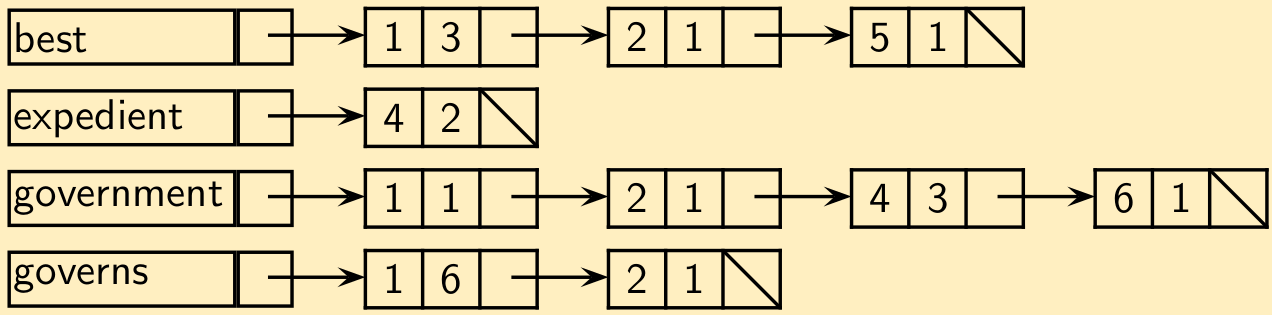
\includegraphics[width=\linewidth]{mem-based}
    \end{block}

    \begin{columns}[T]
        \column<2->{0.48\textwidth}

        \begin{exampleblock}{Time requirements}
            \small
            \begin{tabular}{cc@{~}c@{~}c}
                $T =$ & $Bt_r + Ft_p$ & $+$ & $I(t_d + t_r)$ \\
                & $\uparrow$ & & $\uparrow$ \\
                & parse text & & write file \\
            \end{tabular}
            \emph{$\approx 6h$}
        \end{exampleblock}

        \column<2->{0.48\textwidth}

        \only<2>{\tiny
      \begin{tabular}{l}
          $B = \text{text size}$\\
          $F = \text{n. terms}$\\
          $t_r = \text{transfer rate}$\\
          $t_p = \text{parse time}$ \\
          $I = \text{file size}$ \\
          $t_d = \text{coding time}$
      \end{tabular}
    }

    \only<3>{
        \begin{exampleblock}{Space requirements}
            \footnotesize
            \begin{tabular}{cc@{~}c@{~}c}
                $S =$ & $(4+4+2)$ & $\times$ & $400\,000\,000$ \\
                & $\uparrow$ & & $\uparrow$ \\
                & pointer size & & n. of pointers
            \end{tabular}
            \emph{$\approx 4 Gb$}
        \end{exampleblock}
}
    \end{columns}

\end{frame}

% ----------------------------------------------------------------------

\section{Sort-based Inversion}

\begin{frame}
    \frametitle{Sort-based Inversion}
    
    \begin{block}{}
        \begin{itemize}
        \item If virtual memory was used, the dictionary-based algorithm would take
            about \emph{6 weeks} to index the 5 Gbyte collection
        \item Mainly due to disk seek time
        \item Solution: allow only \emph{sequential disk access}
        \end{itemize}
    \end{block}

\end{frame}

% ----------------------------------------------------------------------

% \newcounter{num}
\setcounter{num}{0}
% \newcommand{\inum}{\addtocounter{num}{1}\thenum}

\begin{frame}
    \frametitle{Sort-based Inversion Algorithm (I)}
    
    \begin{columns}
        \column{0.49\textwidth}

        \begin{enumerate}
        \item Create an empty dictionary structure $S$;\\
            Create an empty temporary file $T$ on disk;
        \item For each document $D_d$ ($1 \leq d \leq N$):
            \begin{enumerate}
            \item Read and parse $D_d$;
            \item For each triple $\langle t, d, f_{d,t} \rangle$
                \begin{enumerate}
                \item Store $t$ in $S$;
                \item Store $\langle t, d, f_{d,t} \rangle$ in $T$;
                \end{enumerate}
            \end{enumerate}
        \end{enumerate}

        \column{0.49\textwidth}<1->

        \begin{block}{}
            \centering
            \footnotesize
            \begin{tabular}{|lc|}\hline
                \multicolumn{2}{|c|}{$S$} \\\hline
                that & \inum \\
                government & \inum \\
                best & \inum \\
                governs & \inum \\
                least & \inum \\
                ... & \\\hline
            \end{tabular}\hspace{2em}
            \begin{tabular}{|c|}\hline
                $T$ \\\hline
                $\langle 1,1,1 \rangle$ \\
                $\langle 2,1,1 \rangle$ \\
                $\langle 3,1,1 \rangle$ \\
                $\langle 4,1,1 \rangle$ \\
                $\langle 5,1,1 \rangle$ \\
                $\langle 2,2,1 \rangle$ \\
                $\langle 3,2,1 \rangle$ \\
                $\langle 4,2,1 \rangle$ \\
                $\langle 5,3,1 \rangle$ \\
                $\langle 6,3,2 \rangle$ \\
                ... \\\hline
            \end{tabular}      
        \end{block}
    \end{columns}
\end{frame}

% ----------------------------------------------------------------------

\begin{frame}
    \frametitle{Sort-based Inversion Algorithm (II)}
    
    \begin{columns}
        \column{0.49\textwidth}

        \begin{enumerate}
            \setcounter{enumi}{2}
        \item Le $k$ be the number of records that fit in memory
            \begin{enumerate}
            \item Read $k$ records from $T$;
            \item Sort according to $t$ and $d$;
            \item Write the sorted run into $T$;
            \item Repeat until all runs are sorted;
            \end{enumerate}
        \item Pairwise merge the sorted runs;
        \end{enumerate}

        \column{0.49\textwidth}

        \begin{block}{}
            \centering \small

            \only<1>{
              \begin{tabular}{|c|}\hline
                  $T$ \\\hline
                  $\langle 1,1,1 \rangle$ \\
                  $\langle 2,1,1 \rangle$ \\
                  $\langle 3,1,1 \rangle$ \\
                  $\langle 4,1,1 \rangle$ \\
                  $\langle 5,1,1 \rangle$ \\
                  $\langle 2,2,1 \rangle$ \\
                  $\langle 3,2,1 \rangle$ \\
                  $\langle 4,2,1 \rangle$ \\
                  $\langle 5,3,1 \rangle$ \\
                  $\langle 6,3,2 \rangle$ \\
                  ... \\\hline
              \end{tabular}      
              {\large $\rightarrow$}
              \begin{tabular}{|c|}\hline
                  $T$ \\\hline
                  $\langle 1,1,1 \rangle$ \\
                  $\langle 2,1,1 \rangle$ \\
                  $\langle 3,1,1 \rangle$ \\\hline
                  $\langle 2,2,1 \rangle$ \\
                  $\langle 4,1,1 \rangle$ \\
                  $\langle 5,1,1 \rangle$ \\\hline
                  $\langle 3,2,1 \rangle$ \\
                  $\langle 4,2,1 \rangle$ \\
                  $\langle 5,3,1 \rangle$ \\\hline
                  $\langle 6,3,2 \rangle$ \\
                  ... \\\hline
              \end{tabular}      
            }

            \only<2>{
              \begin{tabular}{|c|}\hline
                  $T$ \\\hline
                  $\langle 1,1,1 \rangle$ \\
                  $\langle 2,1,1 \rangle$ \\
                  $\langle 3,1,1 \rangle$ \\\hline
                  $\langle 2,2,1 \rangle$ \\
                  $\langle 4,1,1 \rangle$ \\
                  $\langle 5,1,1 \rangle$ \\\hline
                  $\langle 3,2,1 \rangle$ \\
                  $\langle 4,2,1 \rangle$ \\
                  $\langle 5,3,1 \rangle$ \\\hline
                  $\langle 6,3,2 \rangle$ \\
                  ... \\\hline
              \end{tabular}      
              {\large $\rightarrow$}
              \begin{tabular}{|c|}\hline
                  $T$ \\\hline
                  $\langle 1,1,1 \rangle$ \\
                  $\langle 2,1,1 \rangle$ \\
                  $\langle 2,2,1 \rangle$ \\
                  $\langle 3,1,1 \rangle$ \\
                  $\langle 3,2,1 \rangle$ \\
                  $\langle 4,1,1 \rangle$ \\
                  $\langle 4,2,1 \rangle$ \\
                  $\langle 5,1,1 \rangle$ \\
                  $\langle 5,3,1 \rangle$ \\
                  $\langle 6,3,2 \rangle$ \\
                  ... \\\hline
              \end{tabular}      
            }
        \end{block}
    \end{columns}
\end{frame}

% ----------------------------------------------------------------------

\begin{frame}
    \frametitle{Sort-based Inversion Algorithm (III)}
    
    \begin{columns}
        \column{0.45\textwidth}

        \begin{enumerate}
            \setcounter{enumi}{4}
        \item For each term $t$ ($1 \leq t \leq n$):
            \begin{enumerate}
            \item Start a new inverted file entry;
            \item Read all triples $\langle t, d, f_{d,t} \rangle$ from $T$ and form
                the inverted list of $t$;
            \item Compress the inverted list;
            \item Append the list to the inverted file.
            \end{enumerate}
        \end{enumerate}

        \column{0.6\textwidth}

        \begin{block}{}
            \centering \small

            \begin{tabular}{|c|}\hline
                $T$ \\\hline
                $\langle 1,1,1 \rangle$ \\\hline
                $\langle 2,1,1 \rangle$ \\
                $\langle 2,2,1 \rangle$ \\\hline
                $\langle 3,1,1 \rangle$ \\
                $\langle 3,2,1 \rangle$ \\\hline
                $\langle 4,1,1 \rangle$ \\
                $\langle 4,2,1 \rangle$ \\\hline
                $\langle 5,1,1 \rangle$ \\
                $\langle 5,3,1 \rangle$ \\\hline
                $\langle 6,3,2 \rangle$ \\
                ... \\\hline
            \end{tabular}      
            {\large $\rightarrow$}
            \begin{tabular}{rl}
                $t$ & Inverted list \\\hline
                1 & $\langle 1;(1;1) \rangle$ \\
                2 & $\langle 2;(1;1),(2;1) \rangle$ \\
                3 & $\langle 2;(1;1),(2;1) \rangle$ \\
                4 & $\langle 2;(1;1),(2;1) \rangle$ \\
                5 & $\langle 2;(1;1),(3;1) \rangle$ \\
                6 & $\langle 1;(3;2) \rangle$ \\
                ... & \\
            \end{tabular}
        \end{block}
    \end{columns}
\end{frame}

% ----------------------------------------------------------------------

\newcommand{\ceil}[1]{\ensuremath{\lceil #1 \rceil}}
\newcommand{\floor}[1]{\ensuremath{\lfloor #1 \rfloor}}

\begin{frame}
    \frametitle{Sort-based Inversion Requirements}
    
    \begin{exampleblock}<+->{Time requirements}
        \begin{tabular}{rlcl}
            $T =$ & $Bt_r + Ft_p + 10ft_r$ & $\leftarrow$ & read,parse,write \\
            % 10 <- 10 byte records
            & $+20ft_r + R(1.2k\log k)t_c$ & $\leftarrow$ & sort runs \\
            % 1.2k\log k <- quicksort
            % 20 <- 10 to read + 10 to write
            & $+\ceil{\log R}(20ft_r + ft_c)$ & $\leftarrow$ & merge runs \\
            & $+10ft_r + I(t_d + t_r)$ & $\leftarrow$ & write inverted file \\
            \emph{$\approx 20h$}
        \end{tabular}
    \end{exampleblock}

    \only<1>{
      \tiny
      \begin{tabular}{l}
          $B = \text{text size}$\\
          $t_r = \text{transfer rate}$\\
          $F = \text{total n. terms}$\\
          $t_p = \text{parse time}$ \\
          $f = \text{n. index pointers}$\\
          $R = \text{n. runs}$\\
          $k = \text{size of run}$\\
          $t_c = \text{compare+swap}$ \\
          $I = \text{file size}$ \\
          $t_d = \text{coding time}$
      \end{tabular}
    }

    \begin{exampleblock}<+->{Space requirements}
        \begin{tabular}{cccc}
            $S =$ & $10 \times 400\,000\,000$ & $\times$ & $2$\\
            & $\uparrow$ & & $\uparrow$ \\
            & temp. file size & & plus one copy \\
            \emph{$\approx 8 Gb$}
        \end{tabular}
    \end{exampleblock}

\end{frame}

% ----------------------------------------------------------------------

\begin{frame}
    \frametitle{Compression of the Temporary File}

    \begin{block}{}
        \begin{itemize}
        \item<+-> The $\langle t,d,f_{d,t} \rangle$ triples can be compressed 
            \begin{itemize}
            \item For $\langle d,f_{d,t} \rangle$ we can use methods
                appropriate for index compression (which is another subject
                altogether)
            \item E.g., \emph{Elias-$\delta$} and \emph{unary coding}
            \end{itemize}
        \item<+-> How to code $t$?
        \end{itemize}
    \end{block}

\end{frame}

% ----------------------------------------------------------------------

\begin{frame}
    \frametitle{Using Gaps}

    \begin{block}{}
        \begin{itemize}
        \item Term numbers can be coded as sequences of \emph{$t$-gaps} within each
            \emph{sorted} run
            \begin{center}
                \small
                \begin{tabular}{|c|}
                    ... \\
                    $\langle 2,2,1 \rangle$ \\
                    $\langle 4,1,1 \rangle$ \\
                    $\langle 5,1,1 \rangle$ \\
                    ... \\
                \end{tabular}   
                {\large $\rightarrow$}
                \begin{tabular}{|c|}
                    ... \\
                    $\langle 2,2,1 \rangle$ \\
                    $\langle 3,1,1 \rangle$ \\
                    $\langle 2,1,1 \rangle$ \\
                    ... \\
                \end{tabular}
            \end{center}
        \item A $t$-gap $x$ is encoded as value $x+1$, using \emph{unary coding}
            % \begin{itemize}
            % \item Each run requires a maximum of $k + n$ bits
            % \end{itemize}
        \item The same can be applied for $d$, within the term triples
        \end{itemize}
    \end{block}
\end{frame}

% ----------------------------------------------------------------------

\begin{frame}
    \frametitle{Compression Requirements}

    \vspace{-1ex}

    \begin{exampleblock}<+->{Time requirements}
        \small
        \begin{itemize}
            \setlength{\itemsep}{-1ex}
        \item Runs must be sorted \textit{before writing to disk}
        \item Must share space with dictionary $\Rightarrow$ shorter initial runs
            $\Rightarrow$ more runs to merge
        \item Requirements:
            \begin{tabular}{rlcl}
                $T =$ & $Bt_r + Ft_p$ & $\leftarrow$ & read,parse \\
                & $+R(1.2k\log k)t_c + I'(t_r + t_d)$ & $\leftarrow$ & sort,compress,write \\
                & $\ceil{\log R}(2I'(t_r + t_d) + ft_c)$ & $\leftarrow$ & merge runs \\
                & $(I' + I)(t_r + t_d)$ & $\leftarrow$ & recompress \\
                \emph{$\approx 26h$}
            \end{tabular}
        \end{itemize}
    \end{exampleblock}

    \only<1>{
      \tiny
      \begin{tabular}{l}
          $B = \text{text size}$\\
          $t_r = \text{transfer rate}$\\
          $F = \text{total n. terms}$\\
          $t_p = \text{parse time}$ \\
          $R = \text{n. runs}$\\
          $k = \text{size of run}$\\
          $t_c = \text{compare+swap}$ \\
          $I' = \text{temp. file size}$ \\
          $t_d = \text{coding time}$ \\
          $f = \text{n. index pointers}$\\
          $I = \text{file size}$ \\
      \end{tabular}
    }

    \begin{exampleblock}<+->{Space requirements}
        \small
        \begin{tabular}{ccccccc}
            $S =$ & $(1.1 Mb$ & $+$ & $0.25Mb)$ & $\times$ & $400$ & $\times 2$\\
            & $\uparrow$ & & $\uparrow$ & & $\uparrow$ \\
            & $10^6$ $\langle d,f_{d,t} \rangle$ pairs& & k+n bits & & runs & \\
            & & &  for $t$-gaps & &  (4$\times$ more) & \\
            \emph{$\approx 1 Gb$}
        \end{tabular}    
    \end{exampleblock}

\end{frame}

% ----------------------------------------------------------------------

\section{Multiway Merging}

\begin{frame}
    \frametitle{Multiway Merging}
    
    \begin{block}<+->{}
        \begin{itemize}
        \item The merging process can be improved
        \item Instead of a 2-way merge, use an \emph{$R$-way merge}
            \begin{itemize}
            \item One pass $\Rightarrow$ pointers coded/decoded only once
            \item Increased seek time (+1m, approximately)
            \end{itemize}
        \end{itemize}
    \end{block}

\end{frame}

% ----------------------------------------------------------------------

\begin{frame}
    \frametitle{Multiway Merging}

    \begin{exampleblock}<+->{Time Requirements}
        \small
        \begin{tabular}{rlcl}
            $T =$ & $Bt_r + Ft_p$ & $\leftarrow$ & read,parse \\
            & $+R(1.2k\log k)t_c + I'(t_r + t_d)$ & $\leftarrow$ & sort,compress,write \\
            & $f\ceil{\log R}t_c + I'(t_s/b + t_r + t_d)$ & $\leftarrow$ & merge runs \\
            & $I(t_r + t_d)$ & $\leftarrow$ & recompress \\
            \emph{$\approx 11h$}
        \end{tabular}
    \end{exampleblock}

    \only<1>{
      \tiny
      \begin{tabular}{ll}
          $B = \text{text size}$ & $t_r = \text{transfer rate}$\\
          $F = \text{total n. terms}$ & $t_p = \text{parse time}$ \\
          $R = \text{n. runs}$ & $k = \text{size of run}$\\
          $t_c = \text{compare+swap}$ & $I' = \text{temp. file size}$ \\
          $t_d = \text{coding time}$ & $f = \text{n. index pointers}$\\
          $t_s = \text{seek time}$ & $b\leq M/R = \text{input buffer}$ \\
          $I = \text{file size}$ & \\
      \end{tabular}
    }

    \begin{exampleblock}<+->{Space requirements}
        One copy of the temporary file: \emph{$540 Mb$}
    \end{exampleblock}

\end{frame}

% ----------------------------------------------------------------------

\section{In-place Merging}

\begin{frame}
    \frametitle{In-place Multiway Merging}

    \begin{block}{}
        \begin{itemize}
        \item Assume that runs are split into blocks of $b$ bytes (with added
            padding, if necessary)
        \item R blocks can be read into memory and overwritten by output blocks of
            $b$ bytes
            \begin{itemize}
            \item The output blocks contain the inverted lists
            \item During the process all values can be recoded using the most
                efficient code
            \end{itemize}
        \item If a block overruns the vacant space, it can be appended to the end
            of the file
        \item At the end of the merge, blocks must be sorted
            \begin{itemize}
            \item Block-sorting can be done in linear time, using two $b$-byte
                buffers
            \end{itemize}
        \end{itemize}
    \end{block}


\end{frame}

% ----------------------------------------------------------------------

\begin{frame}
    \frametitle{In-place Multiway Merging}

    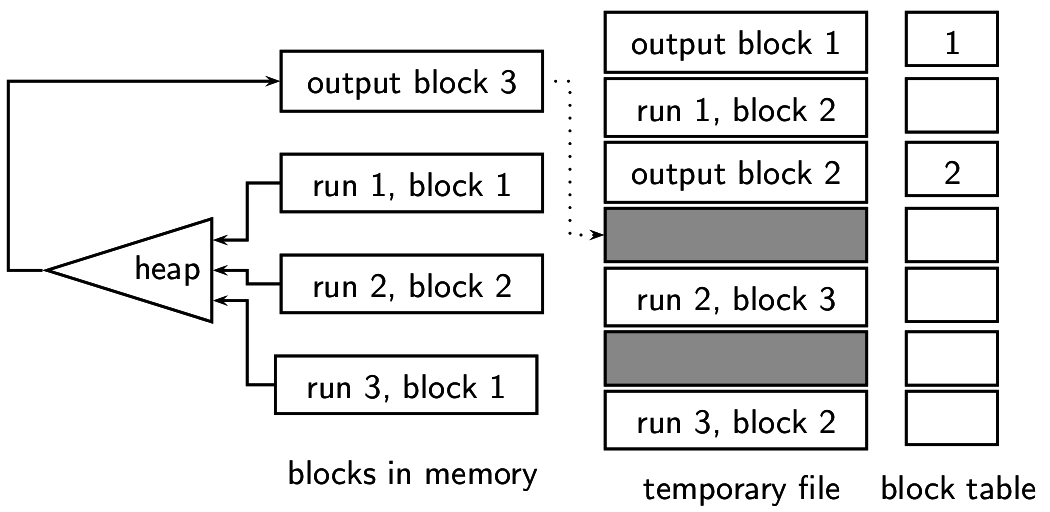
\includegraphics[width=\linewidth]{in-place}

\end{frame}

% ----------------------------------------------------------------------a

\newcommand{\la}{\ensuremath{\leftarrow}}

\begin{frame}
    \frametitle{Block-sorting algorithm}

    For $i$ $\la$ 1 to $nblocks$, if $i \neq blockTable[i]$ then:    
    \begin{enumerate}
    \item Read block $i$ into memory
    \item Set $holding \la blockTable[i]$
    \item Set $vacant \la i$
    \item While $holding \neq vacant$ do
        \begin{enumerate}
        \item Find $j$ such that $blockTable[j] = vacant$
        \item Copy block $j$ to $vacant$
        \item Set $blockTable[vacant] \la vacant$
        \item Set $vacant \la j$
        \end{enumerate}
    \item Write block in memory to $vacant$
    \item Set $blockTable[vacant] \la holding$
    \end{enumerate}
\end{frame}

% ----------------------------------------------------------------------

\begin{frame}
    \frametitle{Multiway Merging Algorithm (I)}
    
    \begin{enumerate}
    \item Initialization:\\
        Create an empty dictionary structure $S$;\\
        Create an empty temporary file $T$ on disk;\\
        Set $L \la |S|$\\
        Set $k \la (M - L)/w$, where $w$ is the number of bytes required to
        store one $\langle t,d,f_{d,t} \rangle$ record\\
        Set $b \la 50 Kb$\\
        Set $R \la 0$\\
    \end{enumerate}
\end{frame}

% ----------------------------------------------------------------------

\begin{frame}
    \frametitle{Multiway Merging Algorithm (II)}
    
    \begin{enumerate}
        \setcounter{enumi}{1}
    \item For each document $D_d$, $1 \leq d \leq N$:
        \begin{enumerate}
        \item Read and parse $D_d$
        \item For each term $t \in D_d$
            \begin{enumerate}
            \item Search $S$ for $t$
            \item If $t$ is not in $S$\\
                insert it\\
                set $L \la |S|$\\
                set $k \la (M-L)/w$
            \item Add a record $\langle t,d,f_{d,t} \rangle$ to the array of triples
            \end{enumerate}
        \item If, at any stage, the array of triples contains $k$ items
            \begin{enumerate}
            \item Sort the array (using quicksort)
            \item Write the array coding $t$-gaps in unary, $d$-gaps with $\delta$ and
                $f_{d,t}$ values in unary
            \item Add padding to complete a block of $b$ bytes
            \item Set $R \la R + 1$
            \item If $(b \times (R+1) > M$, set $b \la b/2$
            \end{enumerate}
        \end{enumerate}
    \end{enumerate}
\end{frame}

% ----------------------------------------------------------------------

\begin{frame}
    \frametitle{Multiway Merging Algorithm (III)}
    
    \begin{enumerate}
        \setcounter{enumi}{2}
    \item Merging:
        \begin{enumerate}
        \item Read the first block from each run and add each block number to
            the free list
        \item Build heap with $R$ candidates (one from each run)
        \item While the heap is non-empty
            \begin{enumerate}
            \item Remove the root
            \item Add it to the output block, recoding
            \item Replace it by the next candidate from the same run
            \end{enumerate}
        \item Each time the output block is full
            \begin{enumerate}
            \item Use the free list to find a vacant space; if there is none, append
                it to the end of the file
            \item Write the output block
            \item Update the free list and block table
            \end{enumerate}
        \item Each time an input block is empty
            \begin{enumerate}
            \item Read the next block from this run
            \item Update the free list
            \end{enumerate}
        \end{enumerate}
    \item Reorder the blocks
    \item Truncate the inverted file
    \end{enumerate}
\end{frame}

% ----------------------------------------------------------------------

\begin{frame}
    \frametitle{Algorithm Requirements}
    
    \begin{exampleblock}<+->{Time Requirements}    
        \small
        \begin{tabular}{rlcl}
            $T =$ & $Bt_r + Ft_p$ & $\leftarrow$ & read,parse \\
            & $+R(1.2k\log k)t_c + I'(t_r + t_d)$ & $\leftarrow$ & sort,compress,write \\
            & $f\ceil{\log R}t_c + (I'+I)(t_s/b + t_r + t_d)$ & $\leftarrow$ & merge,recode \\
            & $2I'(t_s/b + t_r)$ & $\leftarrow$ & permute \\
            \emph{$\approx 11h$}
        \end{tabular}
    \end{exampleblock}

    \only<1>{
      \tiny
      \begin{tabular}{ll}
          $B = \text{text size}$ & $t_r = \text{transfer rate}$\\
          $F = \text{total n. terms}$ & $t_p = \text{parse time}$ \\
          $R = \text{n. runs}$ & $k = \text{size of run}$\\
          $t_c = \text{compare+swap}$ & $I' = \text{temp. file size}$ \\
          $t_d = \text{coding time}$ & $f = \text{n. index pointers}$\\
          $t_s = \text{seek time}$ & $b\leq M/R = \text{input buffer}$ \\
          $I = \text{file size}$ & \\
      \end{tabular}
    }

    \begin{exampleblock}<+->{Space Requirements}
        \small
        Inverted file and temporary file occupy the same space: \emph{150 Mb}
    \end{exampleblock}

\end{frame}

% ----------------------------------------------------------------------

\section{Comparison of Inversion Methods}


\begin{frame}
    \frametitle{Comparison of Inversion Methods}
    
    \begin{block}{}
        \centering
        \small
        \begin{tabular}{lrrr}
            Method & Memory (Mb) & Disk (Mb) & Time (h) \\\hline\hline
            Dictionary-based (mem.) & 4\,000 & 0 & 6 \\
            Dictionary-based (disk) & 30 & 4\,000 & 1\,100 \\
            Sort-based & 40 & 8\,000 & 20 \\
            Sort-based compressed & 40 & 1\,080 & 26 \\
            Multiway merge & 40 & 540 & 11 \\
            In-place multiway merge & 40 & 150 & 11 \\\hline
        \end{tabular}
    \end{block}
\end{frame}

% ----------------------------------------------------------------------

\begin{frame}
    \frametitle{Alternative Inversion Methods}
    
    \begin{block}{Memory-based inversion methods}
        \begin{itemize}
        \item Using \alert{minimal perfect hashing} to eliminate the lexicon from
            memory
        \item Using in-memory compression
        \item Partitioning the inversion process
            \begin{itemize}
            \item Lexicon-based partition
            \item Text-based partition
            \end{itemize}
        \item All these imply several passes through the text
        \end{itemize}
    \end{block}
\end{frame}

% ------------------------------------------------------------

\finalframe{Questions?}

\end{document}
